\section{Manual Prático}:
\subsection{Introdução ao Manual}

\textbf{\medium É importante ressaltar que:}\\[0.4cm]



    Este manual tem caráter prático, dessa forma, não teremos aprofundamento teórico sobre os temas tratados.\\[0.3cm]

    Partimos do pressuposto que a impressora está pronta para uso, isto é, devidamente montada e calibrada.\\[0.3cm]

    Trataremos apenas de impressoras do estilo de produção por fundição por deposição de material(FDM).\\[0.3cm]

    Neste Manual usaremos os Softwares mais comumente utilizados no meio da impressão  3D, o Fusion 360 para a modelagem e o Ultimaker Cura para o fatiamento da peça.\\[0.3cm]

    Não será ensinado a modelar peças do zero, serão apenas ressaltadas mudanças em CAD que otimizam o processo de impressão 3D.\\[0.3cm]

\subsection{Onde tudo começa}:

Antes de começarmos a produzir algo precisamos nos questionar sobre a finalidade daquilo que iremos produzir, tudo possui uma finalidade, um conceito, uma função, seja estética, de acabamento, estrutural, de praticidade, otimização de processo, entre outros exemplos...\\[0.5cm]

\textbf{\Large "O fim da peça dita o começo"}

\subsection{A peça perfeita}

Todos nós estamos à procura da peça perfeita, a peça mais resistente, mais leve, mais bonita, mais produzível, mais barata, entretanto é importante sabermos que esta peça não existe! Bom, não existe como normalmente pensamos, algo que atenda tudo e todos, a peça perfeita que realmente existe é a peça que atende a sua finalidade da melhor maneira possível!


\subsection{Funcionamente de uma impressora 3D}

Para melhor experiência de uso de um equipamento é necessário entender a maneira que o mesmo funciona.\\[0.3cm]

 Simplicando ao máximo, uma impressora 3D atua de forma similar à uma pistola de cola quente que deposita cola sob cola com finalidade de criar um objeto 3D.\\[0.3cm]

Em suma, uma impressora 3D é uma extrusora("pistola de cola quente") controlada numéricamente por computador em torno dos eixos x,y e z. A cabeça de extrusão percorre uma trajetória pré determinada em software enquanto o bico aquecido deposita material derretido, produzindo através de sobposição de camadas, objetos 3D.\\[0.3cm]

\begin{figure}[h!]
    \centering
    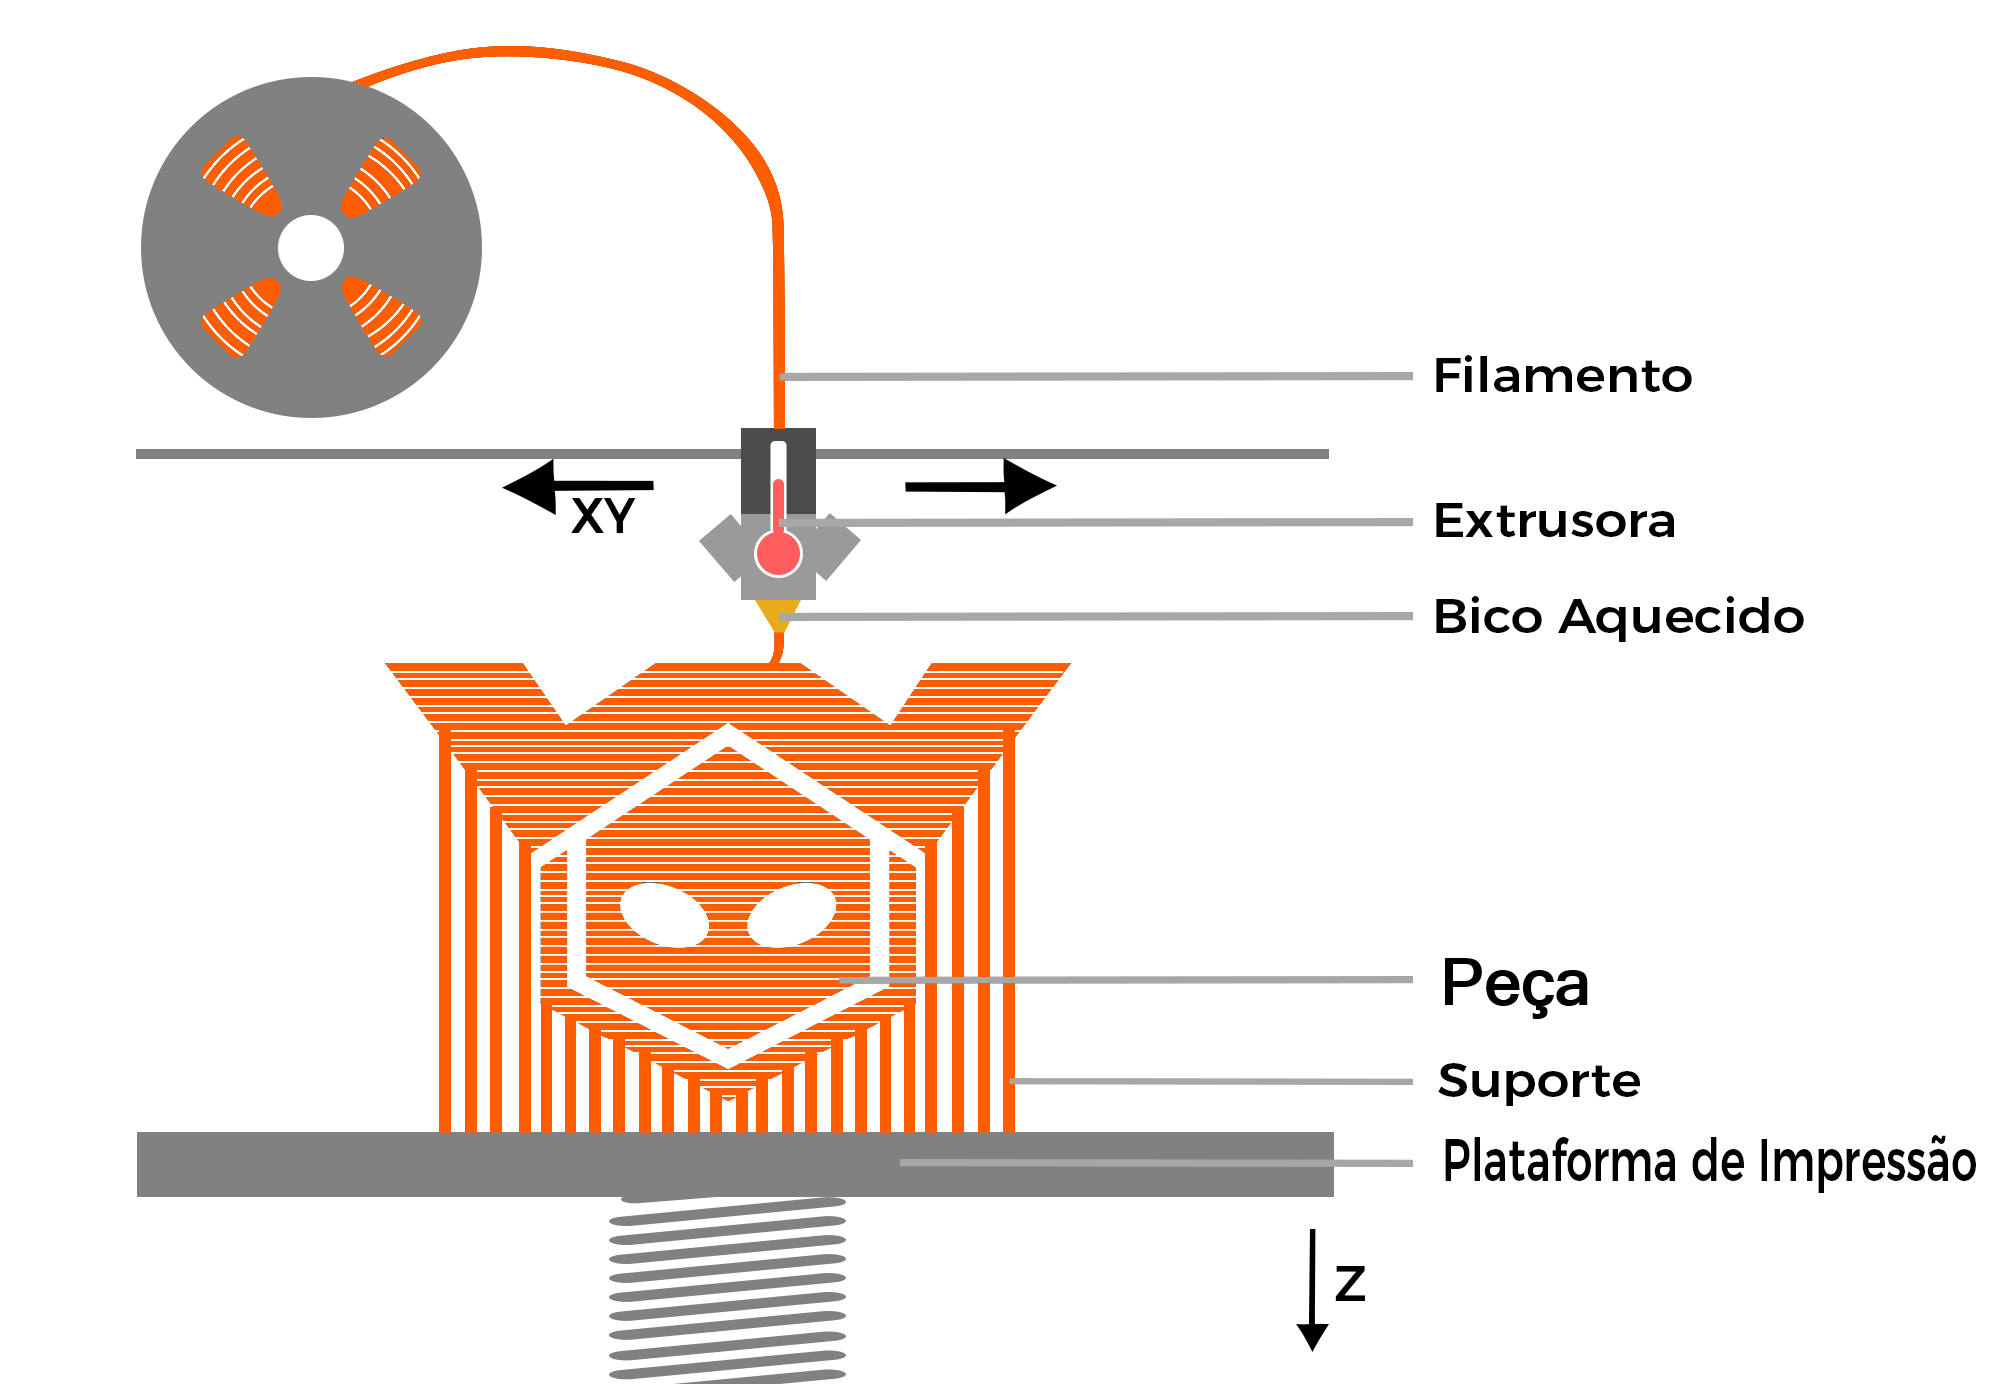
\includegraphics[width=0.45\textwidth]{Fixos/imagens/funcionamento de uma impressora 3D.png}
    \caption{Esquemático do funcionamento de uma impressora 3D}
    \label{fig:my_label}
\end{figure}

\subsection{Softwares necessários}:

Para realizar todo o processo de impressão de uma peça em 3D, é necessário o uso de um software para a modelagem 3D e um para o fatiamento do modelo 3D.\\[0.3cm]
O processo de fatiamento consiste em dividir uma peça em diversas camadas de mesma altura, possibilitando a impressão da mesma.\\[0.3cm]

\begin{figure}[h!]
    \centering
    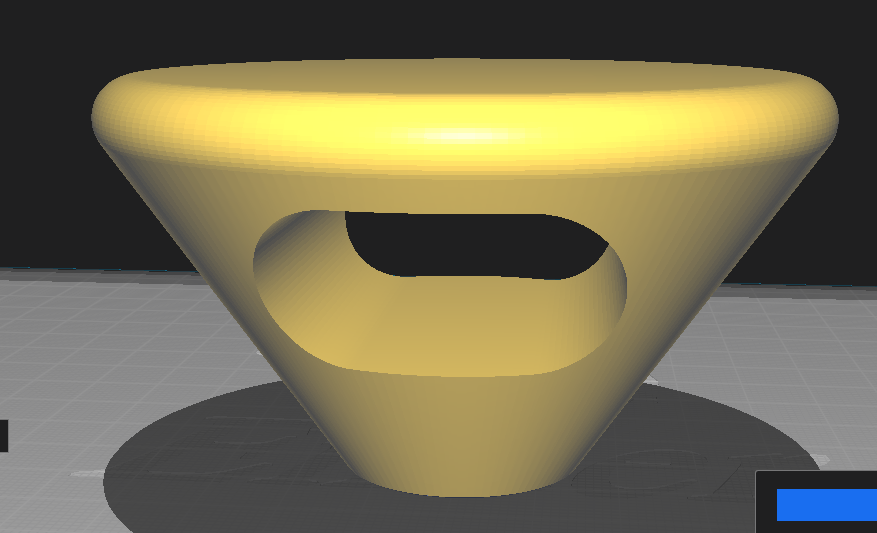
\includegraphics[width=0.25\textwidth]{Fixos/imagens/Modelo 3D v2.png}
    \caption{Peça pré fatiamento}
    \label{fig:my_label}
\end{figure}

\begin{figure}[h!]
    \centering
    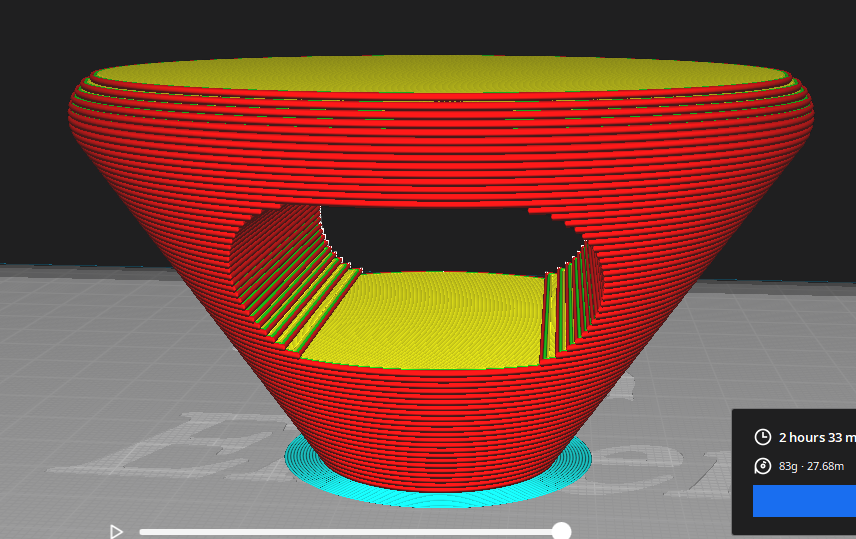
\includegraphics[width=0.25\textwidth]{Fixos/imagens/modelo 3D fatiavdo v2.png}
    \caption{Peça pós fatiamento}
    \label{fig:my_label}
\end{figure}


Neste Manual usaremos os programas mais utilizados entre os usuários de impressoras 3D. O fusion 360 para modelagem e o Ultimaker Cura para o fatiamento.\\[0.3cm]

\subsubsection{Fusion 360}

O fusion 36O é um software de modelagem 3D paramétrica e orgânica criado pela Autodesk, com ele
é possivel criar projetos extremamentes complexos e peças simples.\\[0.3cm]
Possui licença de uso estudantil e de uso Hobbista.\\[0.3cm]

\begin{figure}[h!]
    \centering
    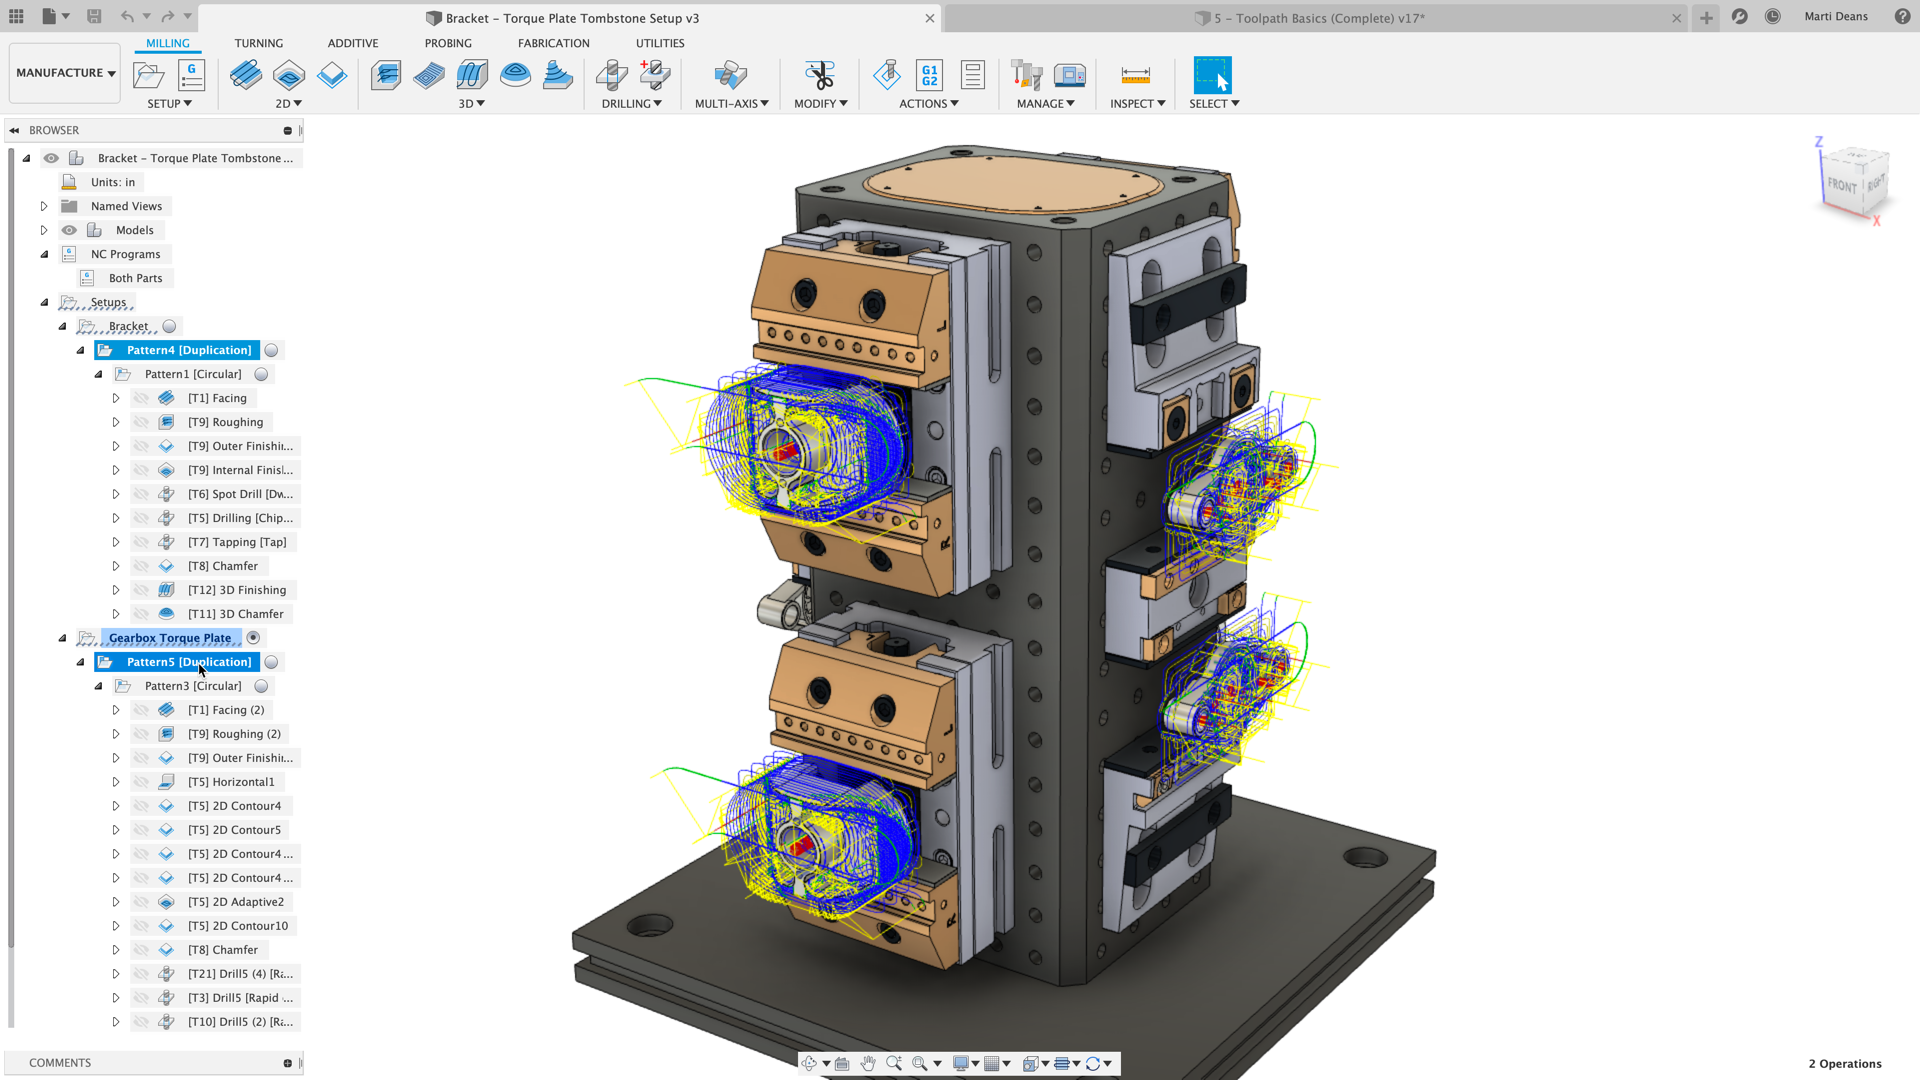
\includegraphics[width=0.35\textwidth]{Fixos/imagens/exemplo fusion.png}
    \caption{Exemplo de projeto criado no Fusion 360}
    \label{fig:my_label}
\end{figure}

Para realizar o download do mesmo basta acessar o link abaixo:\\[0.3cm]

\href{https://www.autodesk.com/products/fusion-360/free-trial}{https://www.autodesk.com/products/fusion-360/free-trial}


\subsubsection{Ultimaker Cura}:

Ultimaker Cura é o software fatiador mais usado do mundo, desenvolvido pela Ultimaker*, com intuito de disseminar a impressão 3D para o público menos técnico, sendo assim, o fatiador mais simples de ser utilizado.\\[0.3cm]

\begin{figure}[h!]
    \centering
    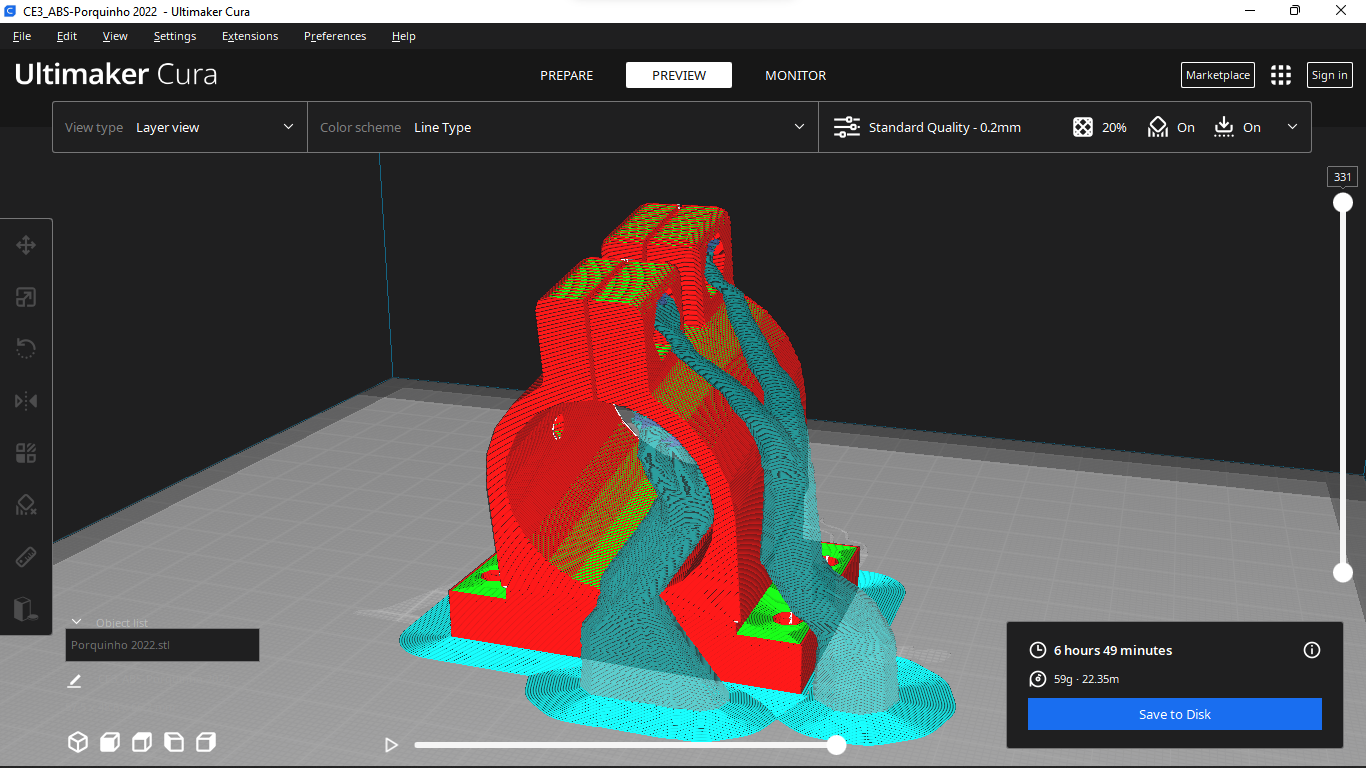
\includegraphics[width=0.35\textwidth]{Fixos/imagens/exemplo cura.png}
    \caption{Exemplo de peça fatiada pelo Cura}
    \label{fig:my_label}
\end{figure}

É possível fazer dowload oficialmente do mesmo através do link:\\[0.3cm]
%
\href{https://ultimaker.com/software/ultimaker-cura}{https://ultimaker.com/software/ultimaker-cura}\\[0.3cm]

*Ultimaker é uma empresa americana dominante no mercado de impressão 3D.
%
\subsection{Processo do CAD}
O processo de criação do modelo 3D é similar aos processo tradicional, entretanto, visando a otimização da impressão 3D é necessário tomar alguns cuidados ao se realizar o CAD.\\[0.3cm]

\subsubsection{Boas práticas dentro do CAD}

\textbf{Dimensionar as estruturas da peça no eixo Z com base em múltiplos da altura de camada}\\[0.3cm]

A altura de camada, como o próprio nome já diz, é a altura de uma camada de material depositada, é necessário que o comprimento no eixo Z da peça seja um múltiplo da altura de camada, caso a divisão entre ambos não seja de resto zero, esta última camada, o resto da divisão, não será depositada, criando assim, uma peça com fuga na dimensão original.\\[0.2cm]

Por exemplo, se criarmos uma peça com 21,3 mm de altura e usarmos uma altura de camada de 0.2 mm, seria necessário 106.5 (21.3 ÷ 0.2 = 106.5) camadas para imprimir por completo a peça, entretanto seriam contabilizadas somente 106 camadas, ficando assim com uma altura de 21,2 mm.`(106 x 0.2 = 21,2)\\[0.3cm]

\textbf{Dimensionar as estruturas da peça nos eixos x e y com base em múltiplos do diâmetro do bico}\\[0.2cm]



Exatamente como ocorre no eixo Z, a divisão entre a largura nos eixos x e y e o diâmetro do bico da extrusora, deve ser de resto zero, caso contrário, a camada restante da divisão não será realizada e o objeto terá fuga dimensional.\\[0.4cm]



\small {Por padrão as impressoras de mesa de impressão ate 33x33 cms usam bico de diâmetro 0.4 mm, em caso de duvida, realize a inspeção visual do componente.\\[0.2cm]



O software fatiador tenta virtualmente compensar camadas de valores "quebrados", entretanto não possui total eficiência}.\\[0.2cm]



\textbf{Trabalhar com ângulos menores de 55 graus} \\[0.2cm]



É intrínseco do processo de impressão 3D que as camadas superiores tenham camadas inferiores para se apoiarem, seguindo essa logica, apenas conseguiríamos imprimir peças sem angulatura alguma, entretanto, é possível sobpocionar camadas de forma a extremidade da camada superior não tenha contato com a inferior, criando assim, ângulos. Essa técnica funciona com ate um angulo limite, o dito, OverHang.\\[0.2cm]



\begin{figure}[h!]

    \centering

    \includegraphics[width=0.25\textwidth]{Fixos/imagens/zoom peça fatiada.png}

    \caption{Camadas com angulatura}

    \label{fig:my_label}

\end{figure}



\begin{figure}[h!]

    \centering

    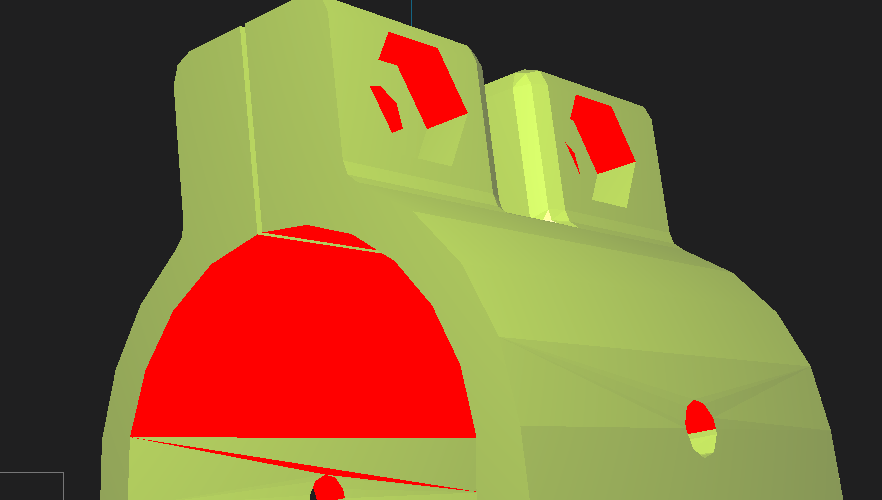
\includegraphics[width=0.25\textwidth]{Fixos/imagens/overhang 2.png}

    \caption{OverHang - Partes em vermelho}

    \label{fig:my_label}

\end{figure}



\textbf{O Overhang depende de cada maquinario, mas em geral está entre 50 e 60 graus}.\\[0.2cm]



Desse modo, é aconselhado que no processo de CAD trabalhe apenas com ângulos menores que 60 graus\\[0.2cm]



Algumas geometrias são apenas possíveis de imprimir com o auxilio de suportes, que são, estruturas criadas durante o processo de impressão com o único intuito de apoiar as partes da peça original que não teriam camadas inferiores para apoio, este tópico será melhor abordado nos parâmetros de impressao.\\[0.2cm]







\subsection{Qual arquivo usar para a impressao?}



Devido ao sistema de movimentação cartesiano, não é possível realizar uma curva em sua real totalidade, desse modo, para imprimir peças com curvaturas, é necessário subdividi-la em diversas retas.\\[0.4cm]



\textbf{\large Todo circulo é um polígono de N lados}\\[0.3cm]



Para imprimir um modelo 3D é necessário converte-lo em uma malha poligonal, o formato .stl ,que significa Standard Triangle Language, no portugues, linguagem universal dos triângulos.\\[0.3cm]

\subsubsection{Salvando em .STL no Fusion 360}



Em geral, os softwares de modelagem 3D já possuem o fomarto .stl em sua aba de:\\[0.3 cm]

"Salvar como" ou "Exportar"\\[0.2cm]



O Fusion 360 possui uma aba exclusiva com essa finalidade.\\[0.3cm]



Basta clicar em FILE --- 3D PRITNG --- Selecionar o objeto que deseja --- OK\\[2cm]



\begin{figure}[h!]

    \centering

    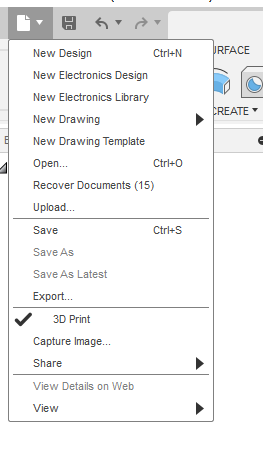
\includegraphics[width=0.25\textwidth]{Fixos/imagens/File 3D printing.png}

    \caption{FILE --> 3D priting}

    \label{fig:my_label}

\end{figure}



\begin{figure}[h!]

    \centering

    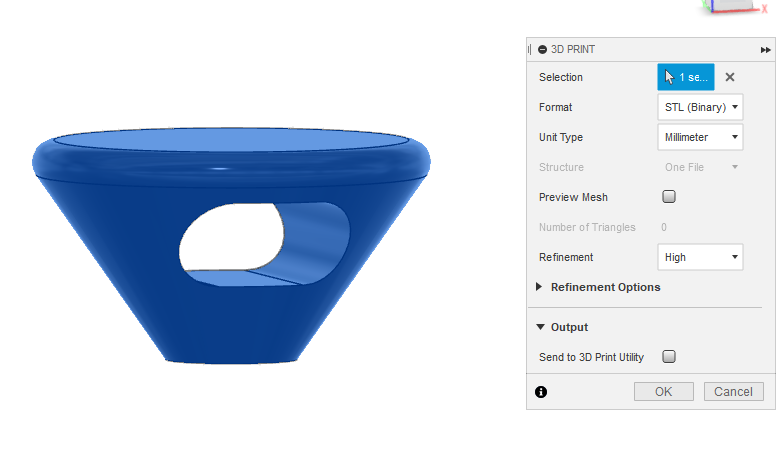
\includegraphics[width=0.25\textwidth]{Fixos/imagens/Objeto salvar como.png}

    \caption{Selecionar o objeto --> Ok}

    \label{fig:my_label}

\end{figure}



\subsection{Escolha do material}

Existem diversos tipos de materias para impressao 3D, entretanto os 3 principais sao:\\[0.4cm]


PLA - Maior facilidade de impressão, menor temperatura de fusão, cerca de 100 reais o KG, baixa resistência a raios UVs, propriedades mecânicas e químicas satisfatórias.\\[0.2cm]



ABS - Maior dificuldade de impressão(requer impressora fechada), temperatura de impressão elevada, cerca de 90 reais o quilo, relativa resistência a raios UVs, propriedades mecânicas e químicas boas, facilidade em acabamento pós impressão (lixar, polir...) \\[0.2cm]



PETG - relativa facilidade de impressão, temperatura de impressão alta, cerca de 130 reais o quilo, boa resistência a raios UVs, propriedades mecânicas e químicas ótimas, relativa facilidade para acabamento pós impressão.\\[0.2cm]

\subsection{Escolha da impressora 3D}



Escolher uma impressora 3D depende basicamente de dois fatores: \\[0.2cm]

o material a ser utilizado e o tamanho da peça. \\[0.2cm]

Alguns materiais possuem uma maior complexidade de impressão, como por exemplo o ABS, que possui uma contração muito alta, por isso, é recomendável impressoras com ambiente de impressão fechado. Policarbonato, PC, por exemplo, possui temperatura de extrusão mais elevadas, sendo necessário impressoras com alta capacidade de aquecimento da extrusora.\\[0.2cm]



Outro fator decisivo, é o volume de impressão, caso a peça seja maior que a área de impressão, não será possível produzi-la no maquinário



Desse modo fica evidente que a capacidade volumétrica de impressão do seu maquinário deve ser compatível com o tamanho das peças que deseja manufaturar.\\[0.2cm]





Entretanto é importante ressaltar que:\\[0.4cm]

\textbf{\large A melhor ferramenta é aquela que nos temos} \\[0.3cm]



Exemplo de impressora com ambiente de impressão Aberto:\\

\begin{figure}[h!]

    \centering

    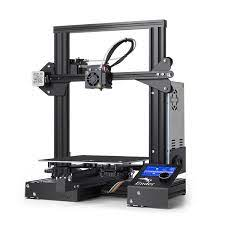
\includegraphics[width=0.25\textwidth]{Fixos/imagens/Ender 3.jpg}

    \caption{Impressora Ender 3}

    \label{fig:my_label}

\end{figure}



Exemplo de impressora com alta capacidade de aquecimento da extrusora:\\



\begin{figure}[h!]

    \centering

    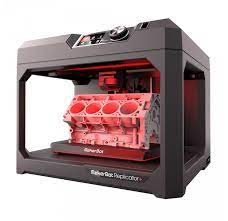
\includegraphics[width=0.25\textwidth]{Fixos/imagens/makerbot replicator.jpg}

    \caption{Impressora Makerbot Replicator}

    \label{fig:my_label}

\end{figure}



Exemplo de impressora com ambiente de impressão fechado:



\begin{figure}[h!]

    \centering

    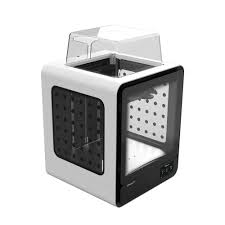
\includegraphics[width=0.25\textwidth]{Fixos/imagens/Cr-200B.jpg}

    \caption{Impressora Cr-200 B}

    \label{fig:my_label}

\end{figure}



\subsection{Configurando o Cura}



\begin{figure}

    \centering[h!]

    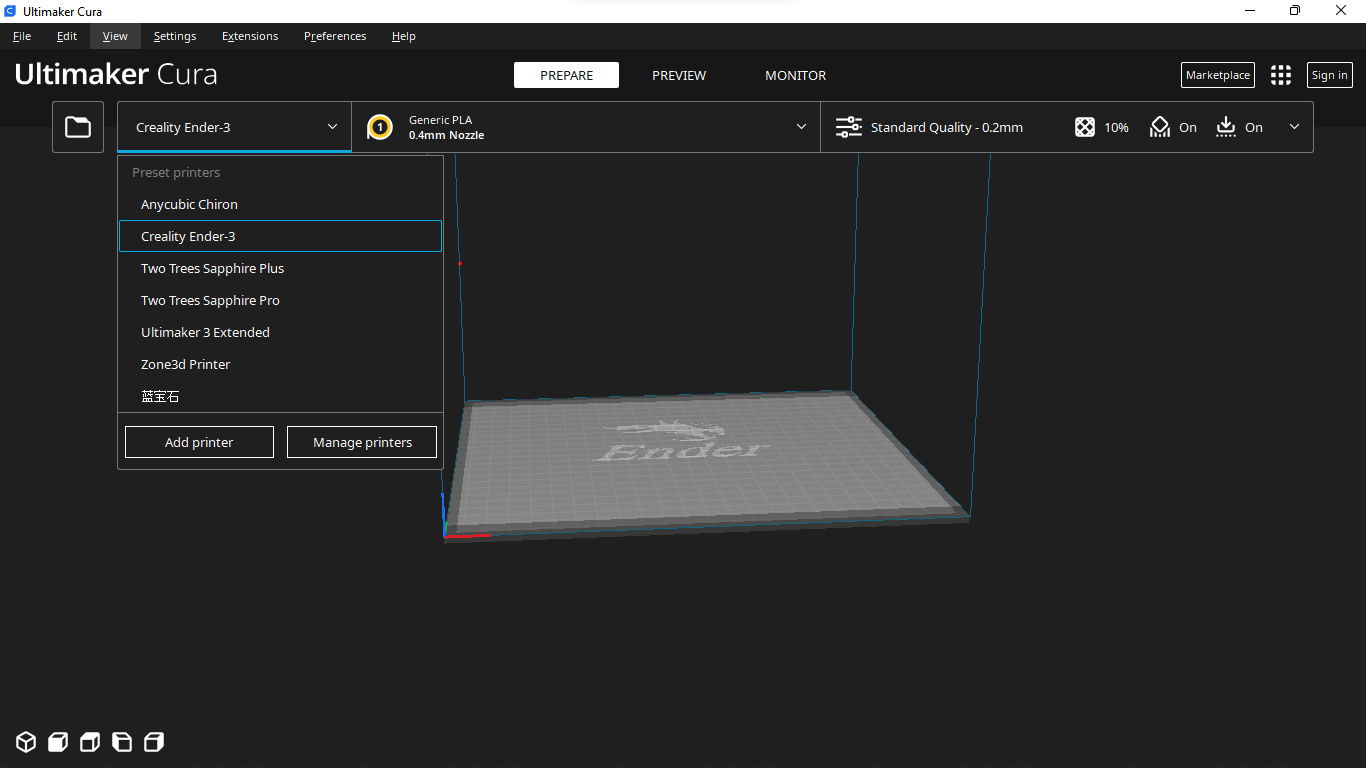
\includegraphics[width=0.45\textwidth]{Fixos/imagens/interface inicial cura.png}

    \caption{Interface inicial do cura}

    \label{fig:my_label}

\end{figure}



Para as configurações iniciais, clicamos no ícone escrito  "PREPARE" no canto superior direito, através dele escolhemos a impressão, o material e alteramos os parâmetros, caso necessário. \\[0.2cm]







\subsubsection{Escolhendo a impressora}

No cura possuímos perfis de impressoras criados pela fabricantes da mesma, esses perfis são basicamente o conjunto de parâmetros ideais para a impressão naquele maquinário.\\[0.2cm]



\subsubsection{Abrindo arquivos}

É possível abrir um ou mais arquivos através ícone em formato de pasta, o primeiro da esquerda para a direita.\\[0.2cm]

\begin{figure}[h!]

    \centering

    
\includegraphics[width=0.65\textwidth]{Fixos/imagens/abaaas cura.png}

    \caption{Abas secundarias do cura}

    \label{fig:my_label}

\end{figure}


\begin{figure}[h!]

    \centering

    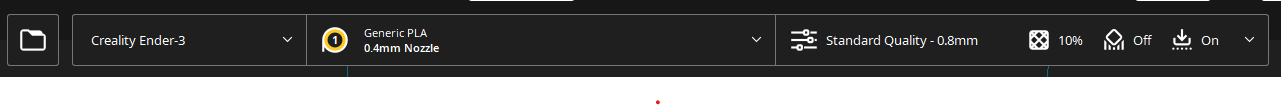
\includegraphics[width=0.65\textwidth]{Fixos/imagens/abas segundarias cura.png}

    \caption{Abas secundarias do cura}

    \label{fig:my_label}

\end{figure}



\begin{figure}[h!]

    \centering

    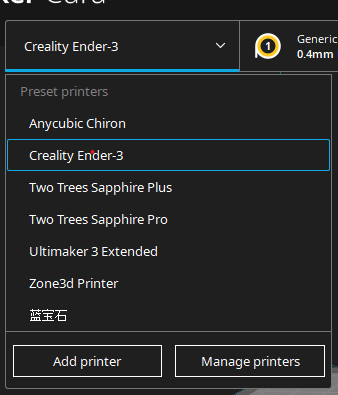
\includegraphics[width=0.45\textwidth]{Fixos/imagens/escolhendo a impressora cura.png}

    \caption{Aba para escolher o perfil da impressora}

    \label{fig:my_label}

\end{figure}



\subsubsection{Escolhendo o material e diâmetxro de bico}

Na figura 15, na segunda fileira é possível ver o local responsável pela escolha do material e o diâmetro do bico.\\[0.2cm]



\subsubsection{Configurando parâmetros}



A terceira coluna da figura 15 diz respeito aos parâmetros de impressão, é possível alterar manualmente qualquer parâmetro que deseje, entretanto focaremos apenas nos mais importantes.\\[0.2cm]



\textbf{Altura de camada}\\[0.2cm]

A altura de camada definira a qualidade superficial da sua peça, em geral, quanto menor a altura mais qualidade e quanto maior menos qualidade, todavia, quanto menor, mais tempo será necessário para a impressão e vice versa.\\



\begin{figure}[h!]

    \centering

    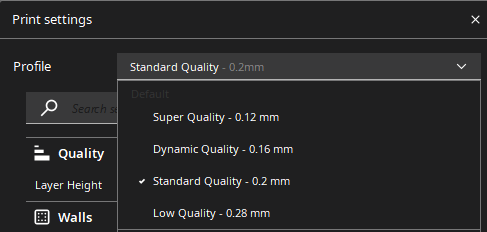
\includegraphics{Fixos/imagens/altura de camada cura.png}

    \caption{Aba responsável pelo valor de altura de camada}

    \label{fig:my_label}

\end{figure}



\small Em geral, a menor altura de camada das impressoras é 0.12 mm\\[0.2cm]



\textbf{Espessura de parede} \\[0.2cm]

É possível configurar a espessura de parede da peça, quantos mais perímetros, mais resistência, entretanto, aumenta-se o peso e o tempo de impressão.\\[0.2cm]



\begin{figure}[h!]

    \centering

    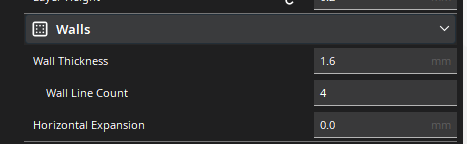
\includegraphics{Fixos/imagens/walls cura.png}

    \caption{Aba responsável pela escolha da espessura de parede}

    \label{fig:my_label}

\end{figure}



\textbf{Preenchimento}

É possível configurar o preenchimento da peça, quantos mais perímetros, mais resistência, entretanto, aumenta-se o peso e o tempo de impressão \\[0.2cm]

Também é possível configurar o padrão de preenchimento da peça \\[0.2cm]



\begin{figure}[h!]

    \centering

    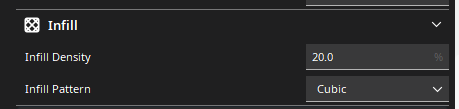
\includegraphics{Fixos/imagens/preenchimento cura.png}

    \caption{Aba responsável pelo valor de preenchimento}

    \label{fig:my_label}

\end{figure}



\textbf{Adesão da peça na mesa}

Em geral usamos duas maneiras de fixação da peça na mesa \\[0.2cm] \\[0.2cm]

Skirt -  imprime-se uma linha com um certo espaçamento ao redor da peça \\[0.2cm]



Brim - Similar ao skit, mas possui contato direto com a peça, sendo necessário sua remoção pôs impressão.  \\[0.2cm]



Em geral, o Skirt tem função apenas de despejar o filamento sobressalente na extrusora de impressões anteriores, já o Brim, aumenta a área de contato da peça na mesa de impressão, sendo necessário em casos que a peça possui pouca área de contato com a mesa, imprimir materiais com a contração alta (ABS).\\[0.2cm]



\textbf{Suporte}



Estrutura usada para sustentar camadas de impressão que originalmente não possuiria apoio, é possível configurar o angulo que começará a ter o uso de suportes, na aba denominada Suport OverHang. \\[0.2cm]



\begin{figure}[h!]

    \centering

    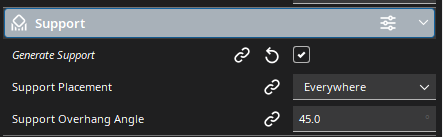
\includegraphics{Fixos/imagens/suport cura.png}

    \caption{Caption}

    \label{fig:my_label}

\end{figure}

.

\subsubsection{Salvando o gcode}

Após realizar o processo de fatiamento, é necessário este arquivo no formato .gcode, que é basicamente as linhas de código que se comunicam diretamente com a impressora.\\[0.2cm]



Para isso basta adicionar a mídia removível do computador, geralmente as impressoras 3D trabalham com cartão microSD e clicar no botão azul escrito "Save removable media" .\\[0.2cm]



\subsection{Imprimindo}

Com sua mídia removível em mãos, basta coloca-la na impressora desejada e em sua interface procurar por "printing for media"

e clicar no arquivo desejado. \\[0.4cm]



Cada interface de maquinário é diferente, entretanto processo é bem similar.\\[0.2cm]


